\begin{figure}[!h]
\centering
\resizebox{\textwidth}{!}{%
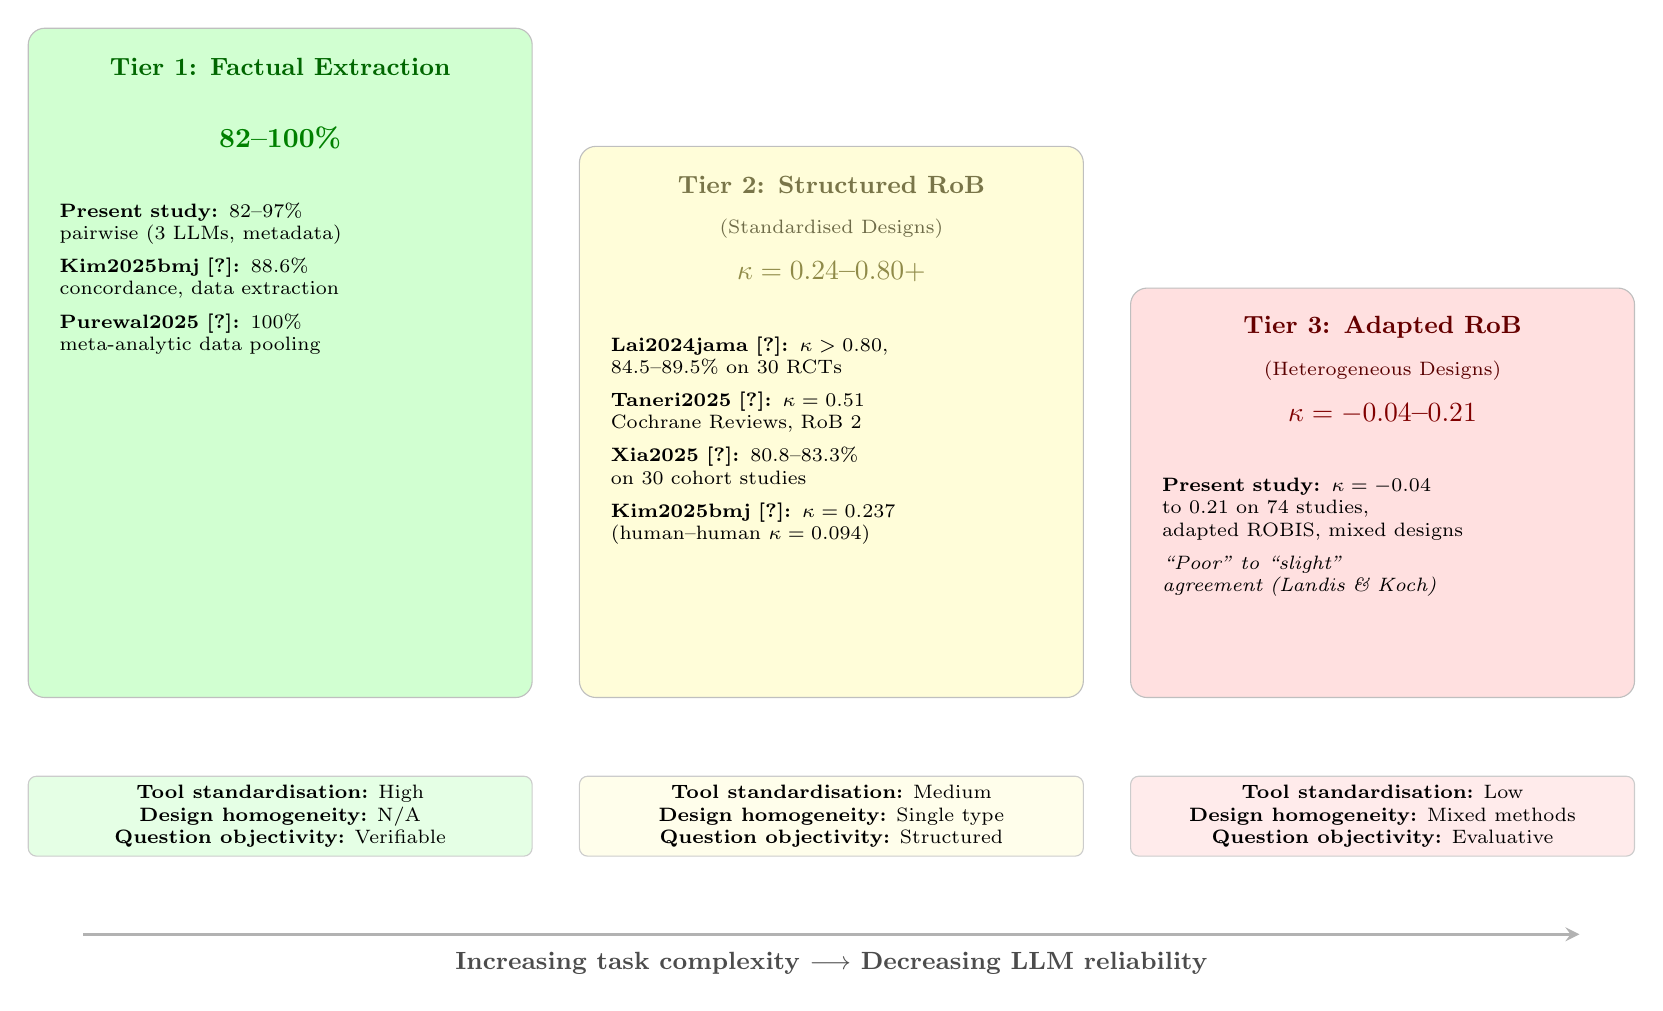
\begin{tikzpicture}[
  tierbox/.style={rectangle, draw=gray!50, rounded corners=6pt,
    minimum width=6.4cm, align=center, font=\small, inner sep=8pt},
  datapt/.style={font=\scriptsize, align=left, text width=5.6cm, anchor=north},
  factbox/.style={rectangle, draw=gray!40, rounded corners=3pt,
    fill=gray!8, minimum width=6.4cm, minimum height=0.8cm,
    align=center, font=\scriptsize},
  arrlabel/.style={font=\small\bfseries, text=black!70},
]

% Horizontal positions
\def\colA{0}
\def\colB{7.0}
\def\colC{14.0}

% Common bottom edge for all tier boxes
\def\ybottom{-3.0}

% ============================================================
% TIER 1 — green, tallest (7.0cm)
% ============================================================
\node[tierbox, fill=green!18, minimum height=8.5cm, anchor=south]
  (t1) at (\colA, \ybottom) {};
\node[font=\small\bfseries, text=green!40!black]
  at ([yshift=-0.5cm]t1.north) {Tier~1: Factual Extraction};
\node[font=\normalsize\bfseries, text=green!50!black]
  at ([yshift=-1.4cm]t1.north) {82--100\%};
\node[datapt] at ([yshift=-2.1cm]t1.north) {%
  \textbf{Present study:} 82--97\%\\pairwise (3~LLMs, metadata)\\[4pt]
  \textbf{\citeauthor{Kim2025bmj}~\cite{Kim2025bmj}:} 88.6\%\\concordance, data extraction\\[4pt]
  \textbf{\citeauthor{Purewal2025}~\cite{Purewal2025}:} 100\%\\meta-analytic data pooling};

% ============================================================
% TIER 2 — yellow, medium height (5.5cm)
% ============================================================
\node[tierbox, fill=yellow!15, minimum height=7.0cm, anchor=south]
  (t2) at (\colB, \ybottom) {};
\node[font=\small\bfseries, text=yellow!40!black]
  at ([yshift=-0.5cm]t2.north) {Tier~2: Structured RoB};
\node[font=\scriptsize, text=yellow!35!black]
  at ([yshift=-1.05cm]t2.north) {(Standardised Designs)};
\node[font=\normalsize\bfseries, text=yellow!50!black]
  at ([yshift=-1.6cm]t2.north) {$\kappa = 0.24$--$0.80+$};
\node[datapt] at ([yshift=-2.3cm]t2.north) {%
  \textbf{\citeauthor{Lai2024jama}~\cite{Lai2024jama}:} $\kappa > 0.80$,\\84.5--89.5\% on 30 RCTs\\[4pt]
  \textbf{\citeauthor{Taneri2025}~\cite{Taneri2025}:} $\kappa = 0.51$\\Cochrane Reviews, RoB~2\\[4pt]
  \textbf{\citeauthor{Xia2025}~\cite{Xia2025}:} 80.8--83.3\%\\on 30 cohort studies\\[4pt]
  \textbf{\citeauthor{Kim2025bmj}~\cite{Kim2025bmj}:} $\kappa = 0.237$\\(human--human $\kappa = 0.094$)};

% ============================================================
% TIER 3 — red, shortest (4.0cm)
% ============================================================
\node[tierbox, fill=red!12, minimum height=5.2cm, anchor=south]
  (t3) at (\colC, \ybottom) {};
\node[font=\small\bfseries, text=red!40!black]
  at ([yshift=-0.5cm]t3.north) {Tier~3: Adapted RoB};
\node[font=\scriptsize, text=red!35!black]
  at ([yshift=-1.05cm]t3.north) {(Heterogeneous Designs)};
\node[font=\normalsize\bfseries, text=red!50!black]
  at ([yshift=-1.6cm]t3.north) {$\kappa = -0.04$--$0.21$};
\node[datapt] at ([yshift=-2.3cm]t3.north) {%
  \textbf{Present study:} $\kappa = -0.04$\\to $0.21$ on 74 studies,\\adapted ROBIS, mixed designs\\[4pt]
  {\itshape``Poor'' to ``slight''\\agreement (Landis \& Koch)}};

% ============================================================
% THREE-FACTOR MODEL (below tiers)
% ============================================================
\def\yfact{-4.5}

\node[factbox, fill=green!10] at (\colA, \yfact) {%
  \textbf{Tool standardisation:} High\\
  \textbf{Design homogeneity:} N/A\\
  \textbf{Question objectivity:} Verifiable};

\node[factbox, fill=yellow!8] at (\colB, \yfact) {%
  \textbf{Tool standardisation:} Medium\\
  \textbf{Design homogeneity:} Single type\\
  \textbf{Question objectivity:} Structured};

\node[factbox, fill=red!8] at (\colC, \yfact) {%
  \textbf{Tool standardisation:} Low\\
  \textbf{Design homogeneity:} Mixed methods\\
  \textbf{Question objectivity:} Evaluative};

% ============================================================
% BOTTOM ARROW
% ============================================================
\draw[->, >=stealth, very thick, draw=gray!60]
  (\colA - 2.5, -6.0) -- (\colC + 2.5, -6.0);
\node[arrlabel, below] at ({\colB}, -6.1)
  {Increasing task complexity $\longrightarrow$ Decreasing LLM reliability};

\end{tikzpicture}%
}% end resizebox
\caption{The task complexity gradient in LLM-assisted systematic review. LLM reliability decreases predictably from factual extraction (Tier~1) through structured risk-of-bias assessment on standardised designs (Tier~2) to adapted risk-of-bias assessment on heterogeneous educational studies (Tier~3). Data points from the present study (bold) are contextualised against published benchmarks. The gradient is driven by three interacting factors: tool standardisation, study design homogeneity, and question objectivity (see Section~\ref{sec:llm-validation}).}
\label{fig:llm-reliability-gradient}
\end{figure}
